\documentclass[11pt,aspectratio=169]{beamer}

\usetheme[progressbar=frametitle]{metropolis}
\usepackage[utf8]{inputenc}
\usepackage[T1]{fontenc}
\usepackage{amsmath}
\usepackage{amssymb}
\usepackage{mathtools}
\usepackage{booktabs}
\usepackage{tabularx}
\usepackage{array}
\usepackage{colortbl}
\usepackage{tikz}
\usepackage{pgfplots}
\pgfplotsset{compat=1.18}
\usetikzlibrary{shapes.geometric, arrows.meta, positioning, calc, decorations.pathreplacing, patterns}
\usepackage{graphicx}
\usepackage{xcolor}

% ---------- Farben ----------
\definecolor{darkblue}{HTML}{1F3864}
\definecolor{midblue}{HTML}{2E5090}
\definecolor{lightblue}{HTML}{E8EEF6}
\definecolor{accentblue}{HTML}{3B8BD4}
\definecolor{mygreen}{HTML}{1A7A1A}
\definecolor{lightgreen}{HTML}{EAF3DE}
\definecolor{myred}{HTML}{A32D2D}
\definecolor{lightred}{HTML}{FCEBEB}
\definecolor{amber}{HTML}{854F0B}

\setbeamercolor{palette primary}{bg=darkblue,fg=white}
\setbeamercolor{progress bar}{fg=accentblue,bg=lightblue}
\setbeamercolor{frametitle}{bg=darkblue,fg=white}

% ---------- Hilfskommandos ----------
\newcommand{\guard}[1]{g_{#1}}
\newcommand{\svar}[2]{s_{#1,#2}}

% L-Polygon TikZ Macro (roter Faden)
\newcommand{\lpolygon}[1][1.0]{%
  \begin{tikzpicture}[scale=#1]
    \fill[lightblue!60] (0,2)--(1,2)--(1,1)--(2,1)--(2,0)--(0,0)--cycle;
    \draw[darkblue, thick] (0,2)--(1,2)--(1,1)--(2,1)--(2,0)--(0,0)--cycle;
    \foreach \x/\y/\name/\pos in {
      0/2/v_1/left, 1/2/v_2/above, 1/1/v_3/above right,
      2/1/v_4/right, 2/0/v_5/right, 0/0/v_6/left}{
      \fill[darkblue] (\x,\y) circle (2.2pt);
      \node[\pos, font=\tiny, darkblue] at (\x,\y) {$\name$};
    }
  \end{tikzpicture}%
}

% ---------- Titel ----------
\title{SAT- und MaxSAT-Enkodierung des Art Gallery Problems}
\subtitle{Methodik, Implementierung und Benchmark-Ergebnisse}
\author{Elena Berschauer}
\institute{Lehrstuhl für Rechnerarchitektur \\
Betreuer: Mathias Fleury}
\date{17. Juni 2026}

\begin{document}

% ============================================================
\begin{frame}
  \titlepage
\end{frame}
% ============================================================

\begin{frame}{Inhalt}
  \tableofcontents
\end{frame}

% ============================================================
\section{Art Gallery Problem}
% ============================================================

\begin{frame}{Warum AGP lösen?}
  \begin{columns}[T]
    \begin{column}{0.55\textwidth}
      \textbf{Art Gallery Problem (AGP):} Wie viele Wächter (Guards)
      braucht man, um ein Polygon vollständig zu überwachen?
      \vspace{0.6em}

      \begin{block}{Praktische Relevanz}
        Kameraplatzierung, Sensornetze, Roboternavigation
      \end{block}
      \vspace{0.3em}
      \begin{block}{Theoretische Tiefe}
        Klassisches Problem der Computational Geometry,
        \textbf{NP-schwer} (Lee \& Lin, 1986)
      \end{block}
      \vspace{0.3em}
      \begin{alertblock}{Ziel}
        Das \emph{Minimum} an Guards finden, beweisbar optimal,
        nicht nur eine obere Schranke. $\Rightarrow$ SAT
      \end{alertblock}
    \end{column}
    \begin{column}{0.42\textwidth}
      \centering
      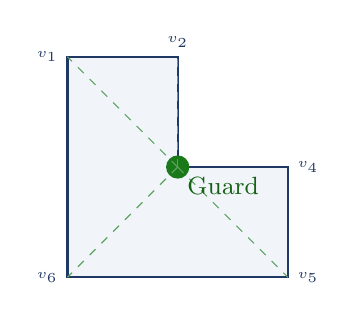
\begin{tikzpicture}[scale=1.4]
        \fill[lightblue!60] (0,2)--(1,2)--(1,1)--(2,1)--(2,0)--(0,0)--cycle;
        \draw[darkblue, thick] (0,2)--(1,2)--(1,1)--(2,1)--(2,0)--(0,0)--cycle;
        % Guard at p3=(1,1)
        \fill[mygreen] (1,1) circle (3pt);
        \draw[mygreen!70, dashed, thin] (1,1)--(0,2);
        \draw[mygreen!70, dashed, thin] (1,1)--(1,2);
        \draw[mygreen!70, dashed, thin] (1,1)--(2,0);
        \draw[mygreen!70, dashed, thin] (1,1)--(0,0);
        \node[mygreen!80!black, font=\small, below right] at (1,1) {Guard};
        \node[darkblue, font=\tiny, left] at (0,2) {$v_1$};
        \node[darkblue, font=\tiny, above] at (1,2) {$v_2$};
        \node[darkblue, font=\tiny, right] at (2,1) {$v_4$};
        \node[darkblue, font=\tiny, right] at (2,0) {$v_5$};
        \node[darkblue, font=\tiny, left] at (0,0) {$v_6$};
      \end{tikzpicture}\\[0.3em]
      \small L-Polygon: 1 Guard genügt
    \end{column}
  \end{columns}
\end{frame}

% =============================================
\section{Pipeline-Überblick}
% =============================================

\begin{frame}{Pipeline-Überblick}
  \centering
  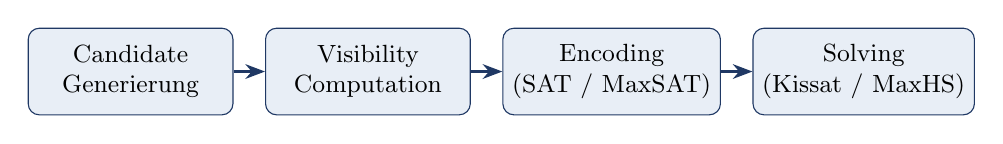
\begin{tikzpicture}[
      node distance=0.4cm,
      box/.style={rectangle, rounded corners, draw=darkblue, fill=lightblue,
                   minimum width=2.6cm, minimum height=1.1cm, align=center, font=\small},
      arrow/.style={-{Stealth[length=2.5mm]}, thick, darkblue}
    ]
    \node[box] (cand) {Candidate\\Generierung};
    \node[box, right=of cand] (vis) {Visibility\\Computation};
    \node[box, right=of vis] (enc) {Encoding\\(SAT / MaxSAT)};
    \node[box, right=of enc] (solve) {Solving\\(Kissat / MaxHS)};

    \draw[arrow] (cand) -- (vis);
    \draw[arrow] (vis) -- (enc);
    \draw[arrow] (enc) -- (solve);
  \end{tikzpicture}
  \vspace{1.5em}
  \begin{itemize}
    \item \textbf{Candidates:} Eckpunkte + relevante Kantenschnittpunkte
    \item \textbf{Visibility:} Sichtbarkeitsmatrix $V$ über Sub-Segment-Dekomposition
    \item \textbf{Encoding:} \alert{Fokus dieses Vortrags}
    \item \textbf{Solving:} Kissat (iterativ) vs.\ MaxHS (direkt)
  \end{itemize}
\end{frame}


% ============================================================
\section{Diskretisierung \& Kandidaten}
% ============================================================

\begin{frame}{Diskretisierung: Warum nicht kontinuierlich?}
  \begin{alertblock}{Problem}
    Das AGP ist über kontinuierliche Flächen definiert —
    SAT kennt nur endlich viele boolesche Variablen.
  \end{alertblock}
  \vspace{0.6em}
  \textbf{Lösung: Diskretisierung}
  \begin{itemize}
    \item Wähle endliche Kandidatenmenge $P \subset \mathbb{R}^2$
    \item Guards und Witnesses stammen beide aus $P$
    \item Coverage wird relativ zu $P$ definiert:
          jeder Punkt in $P$ muss von mindestens einem Guard gesehen werden
  \end{itemize}
  \vspace{0.5em}
  \begin{block}{Guards = Witnesses}
    In dieser Implementierung ist $P$ sowohl die Menge möglicher Guard-Positionen
    als auch die Menge der zu überwachenden Witness-Punkte.\\
    Konsequenz: Sichtbarkeitsmatrix $V$ ist \emph{symmetrisch}, $V[i][i]=1$.
  \end{block}
\end{frame}

\begin{frame}{Kandidatengenerierung}
  \begin{columns}[T]
    \begin{column}{0.50\textwidth}
      \textbf{Welche Punkte werden gewählt?}
      \begin{enumerate}
        \item Alle Eckpunkte des Polygons ($P_0$)
        \item Nur \emph{sichtbare} Eckenpaare $v_i, v_j$ betrachten:
              $\overline{v_i v_j} \subseteq \bar{P}$
        \item Schnittpunkte dieser Sichtlinien mit Kanteninneren
              werden zu $P_1$ hinzugefügt
      \end{enumerate}
      \vspace{0.5em}
      \textbf{Warum nur sichtbare Paare?}\\
      Eine Gerade durch zwei Ecken, die sich nicht sehen, verlässt
      das Polygon — ihre Schnittpunkte sind geometrisch nicht relevant
      für die Sichtbarkeitsstruktur.
    \end{column}
    \begin{column}{0.47\textwidth}
      \centering
      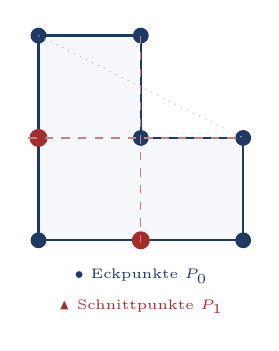
\begin{tikzpicture}[scale=1.3]
        \fill[lightblue!40] (0,2)--(1,2)--(1,1)--(2,1)--(2,0)--(0,0)--cycle;
        \draw[darkblue, thick] (0,2)--(1,2)--(1,1)--(2,1)--(2,0)--(0,0)--cycle;
        % Eckpunkte (P0)
        \foreach \x/\y in {0/2, 1/2, 1/1, 2/1, 2/0, 0/0}{
          \fill[darkblue] (\x,\y) circle (2.2pt);
        }
        % Kandidaten P1 (nur 2 Schnittpunkte)
        \foreach \x/\y in {1/0, 0/1}{
          \fill[myred] (\x,\y) circle (2.5pt);
        }
        % Sichtlinien die Schnittpunkte erzeugen
        \draw[myred!60, dashed, thin] (1,2)--(1,-0.1);
        \draw[myred!60, dashed, thin] (-0.1,1)--(2,1);
        % Beispiel nicht sichtbares Paar (gestrichelt grau, durchgestrichen)
        \draw[gray!50, dotted, thin] (0,2)--(2,1);
        \node[font=\tiny, darkblue] at (1.0,-0.35) {$\bullet$ Eckpunkte $P_0$};
        \node[font=\tiny, myred] at (1.0,-0.65) {$\blacktriangle$ Schnittpunkte $P_1$};
      \end{tikzpicture}
    \end{column}
  \end{columns}
\end{frame}

\begin{frame}{L-Polygon: 15 Eckenpaare $\to$ 8 Kandidaten}
  \begin{columns}[T]
    \begin{column}{0.52\textwidth}
      \begin{enumerate}
        \item $\binom{6}{2}=15$ mögliche Eckenpaare
        \item Mittelpunkttest: nur \textbf{12} Paare sichtbar
              (3 verlassen das Polygon, z.\,B.\ $v_1{\to}v_4$)
        \item Von den 12 Sichtlinien liefern nur \textbf{2}
              neue Schnittpunkte im Kanteninneren
      \end{enumerate}
      \vspace{0.5em}
      \begin{block}{L-Polygon: finale Kandidatenmenge}
        \begin{tabular}{lc}
          \toprule
          Quelle & Anzahl \\
          \midrule
          Eckpunkte $P_0$ & 6 \\
          Schnittpunkte $P_1$ & 2 \\
          \midrule
          $|P|$ gesamt & \textbf{8} \\
          \bottomrule
        \end{tabular}
      \end{block}
    \end{column}
    \begin{column}{0.45\textwidth}
      \centering
      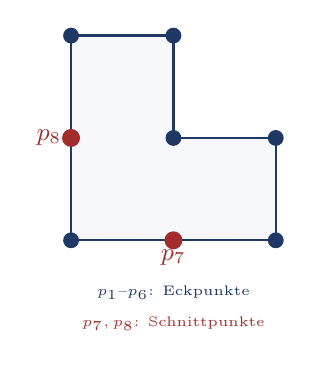
\begin{tikzpicture}[scale=1.3]
        \fill[lightblue!40] (0,2)--(1,2)--(1,1)--(2,1)--(2,0)--(0,0)--cycle;
        \draw[darkblue, thick] (0,2)--(1,2)--(1,1)--(2,1)--(2,0)--(0,0)--cycle;
        \foreach \x/\y in {0/2, 1/2, 1/1, 2/1, 2/0, 0/0}{
          \fill[darkblue] (\x,\y) circle (2.2pt);
        }
        \fill[myred] (1,0) circle (2.5pt);
        \node[below, font=\small, myred] at (1,0) {$p_7$};
        \fill[myred] (0,1) circle (2.5pt);
        \node[left, font=\small, myred] at (0,1) {$p_8$};
        \node[font=\tiny, darkblue, below] at (1,-0.35) {$p_1$--$p_6$: Eckpunkte};
        \node[font=\tiny, myred, below] at (1,-0.65) {$p_7,p_8$: Schnittpunkte};
      \end{tikzpicture}\\[0.2em]
      \small $p_7=(1,0)$: Linie $v_2v_3 \cap e_5$\\
      $p_8=(0,1)$: Linie $v_3v_4 \cap e_6$
    \end{column}
  \end{columns}
\end{frame}

% ============================================================
\section{Sichtbarkeit}
% ============================================================

\begin{frame}{Sichtbarkeitsdefinition}
  \begin{block}{Definition}
    Guard $p_i$ sieht Witness $p_j$ genau dann, wenn die Strecke
    $\overline{p_i p_j}$ vollständig in der abgeschlossenen Hülle
    $\bar{P} = P^\circ \cup \partial P$ liegt.
  \end{block}
  \vspace{0.6em}
  \textbf{Wichtige Randfälle:}
  \begin{itemize}
    \item \textbf{Kanten sind sichtbar:} Strecken entlang des Randes zählen als sichtbar
          ($\overline{P}$ ist \emph{abgeschlossen})
    \item \textbf{Reflex-Vertex:} Sichtlinie darf einen Reflex-Vertex
          berühren, solange sie das Polygoninnere nicht verlässt —
          in dieser Implementierung gilt das als sichtbar
    \item \textbf{Numerische Toleranz:} $\varepsilon = 10^{-6}$ für Floating-Point-Vergleiche
  \end{itemize}

\end{frame}

\begin{frame}{Sichtbarkeitsmatrix $V$ — L-Polygon ($|P|=8$)}
  \begin{columns}[T]
    \begin{column}{0.36\textwidth}
      \centering
      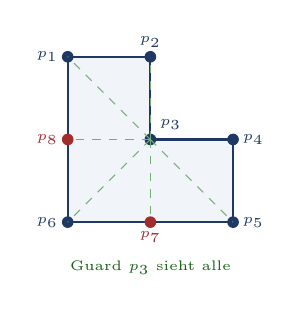
\begin{tikzpicture}[scale=1.05]
        \fill[lightblue!60] (0,2)--(1,2)--(1,1)--(2,1)--(2,0)--(0,0)--cycle;
        \draw[darkblue, thick] (0,2)--(1,2)--(1,1)--(2,1)--(2,0)--(0,0)--cycle;
        \foreach \x/\y/\name/\pos in {
          0/2/p_1/left, 1/2/p_2/above, 1/1/p_3/above right,
          2/1/p_4/right, 2/0/p_5/right, 0/0/p_6/left}{
          \fill[darkblue] (\x,\y) circle (2pt);
          \node[\pos, font=\tiny, darkblue] at (\x,\y) {$\name$};
        }
        \fill[myred] (1,0) circle (2pt);
        \node[below, font=\tiny, myred] at (1,0) {$p_7$};
        \fill[myred] (0,1) circle (2pt);
        \node[left, font=\tiny, myred] at (0,1) {$p_8$};
        % p3 sieht alles
        \draw[mygreen!60, dashed, thin] (1,1)--(0,2);
        \draw[mygreen!60, dashed, thin] (1,1)--(1,2);
        \draw[mygreen!60, dashed, thin] (1,1)--(2,0);
        \draw[mygreen!60, dashed, thin] (1,1)--(0,0);
        \draw[mygreen!60, dashed, thin] (1,1)--(1,0);
        \draw[mygreen!60, dashed, thin] (1,1)--(0,1);
        \node[mygreen!80!black, font=\tiny, below] at (1,-0.35) {Guard $p_3$ sieht alle};
      \end{tikzpicture}\\[0.3em]
      \small $|P|=8$\\
      ($p_1$--$p_6$ Ecken, $p_7,p_8$ Schnittpunkte)
    \end{column}
    \begin{column}{0.60\textwidth}
      \small $V[i][j]=1 \iff \overline{p_i p_j} \subseteq \bar{P}$
      \vspace{0.3em}

      \setlength{\tabcolsep}{3.5pt}
      \begin{tabular}{c|cccccccc}
        \toprule
         & $p_1$ & $p_2$ & $p_3$ & $p_4$ & $p_5$ & $p_6$ & $p_7$ & $p_8$ \\
        \midrule
        $p_1$ & \cellcolor{lightgreen!70}1 & \cellcolor{lightgreen!70}1 & \cellcolor{lightgreen!70}1 & 0 & \cellcolor{lightgreen!70}1 & \cellcolor{lightgreen!70}1 & \cellcolor{lightgreen!70}1 & \cellcolor{lightgreen!70}1 \\
        $p_2$ & \cellcolor{lightgreen!70}1 & \cellcolor{lightgreen!70}1 & \cellcolor{lightgreen!70}1 & 0 & 0 & \cellcolor{lightgreen!70}1 & \cellcolor{lightgreen!70}1 & \cellcolor{lightgreen!70}1 \\
        $p_3$ & \cellcolor{lightgreen!70}1 & \cellcolor{lightgreen!70}1 & \cellcolor{lightgreen!70}1 & \cellcolor{lightgreen!70}1 & \cellcolor{lightgreen!70}1 & \cellcolor{lightgreen!70}1 & \cellcolor{lightgreen!70}1 & \cellcolor{lightgreen!70}1 \\
        $p_4$ & 0 & 0 & \cellcolor{lightgreen!70}1 & \cellcolor{lightgreen!70}1 & \cellcolor{lightgreen!70}1 & \cellcolor{lightgreen!70}1 & \cellcolor{lightgreen!70}1 & \cellcolor{lightgreen!70}1 \\
        $p_5$ & \cellcolor{lightgreen!70}1 & 0 & \cellcolor{lightgreen!70}1 & \cellcolor{lightgreen!70}1 & \cellcolor{lightgreen!70}1 & \cellcolor{lightgreen!70}1 & \cellcolor{lightgreen!70}1 & \cellcolor{lightgreen!70}1 \\
        $p_6$ & \cellcolor{lightgreen!70}1 & \cellcolor{lightgreen!70}1 & \cellcolor{lightgreen!70}1 & \cellcolor{lightgreen!70}1 & \cellcolor{lightgreen!70}1 & \cellcolor{lightgreen!70}1 & \cellcolor{lightgreen!70}1 & \cellcolor{lightgreen!70}1 \\
        $p_7$ & \cellcolor{lightgreen!70}1 & \cellcolor{lightgreen!70}1 & \cellcolor{lightgreen!70}1 & \cellcolor{lightgreen!70}1 & \cellcolor{lightgreen!70}1 & \cellcolor{lightgreen!70}1 & \cellcolor{lightgreen!70}1 & \cellcolor{lightgreen!70}1 \\
        $p_8$ & \cellcolor{lightgreen!70}1 & \cellcolor{lightgreen!70}1 & \cellcolor{lightgreen!70}1 & \cellcolor{lightgreen!70}1 & \cellcolor{lightgreen!70}1 & \cellcolor{lightgreen!70}1 & \cellcolor{lightgreen!70}1 & \cellcolor{lightgreen!70}1 \\
        \bottomrule
      \end{tabular}
      \vspace{0.5em}

      \small
      $p_3, p_6, p_7, p_8$: vollständige Zeile $\Rightarrow$ sehen alle 8 Punkte\\[0.2em]
      $V[1][4]=0$: $p_1{\to}p_4$ verlässt das Polygon
    \end{column}
  \end{columns}
\end{frame}



\begin{frame}{Sub-Segment-Dekomposition}
  \begin{columns}[T]
    \begin{column}{0.48\textwidth}
      \textbf{Naiver Mittelpunkttest: Falsch positiv}\\[0.4em]
      Segment von $(0,5)$ zu $(4,5)$ im U-Polygon:\\[0.4em]
      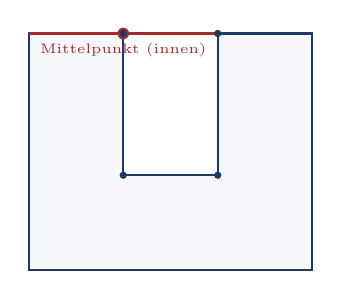
\begin{tikzpicture}[scale=0.6]
        % U-Polygon
        \fill[lightblue!40] (0,0)--(6,0)--(6,5)--(4,5)--(4,2)--(2,2)--(2,5)--(0,5)--cycle;
        \draw[darkblue,thick] (0,0)--(6,0)--(6,5)--(4,5)--(4,2)--(2,2)--(2,5)--(0,5)--cycle;
        % Segment
        \draw[myred, thick] (0,5)--(4,5);
        % Mittelpunkt
        \fill[myred] (2,5) circle (3.5pt);
        \node[myred, font=\tiny, below] at (2,5) {Mittelpunkt (innen)};
        % Vertikale Kanten
        \fill[darkblue] (2,5) circle (2.2pt);
        \fill[darkblue] (2,2) circle (2.2pt);
        \fill[darkblue] (4,5) circle (2.2pt);
        \fill[darkblue] (4,2) circle (2.2pt);
      \end{tikzpicture}\\[0.2em]
      \small Mittelpunkt $(2,5)$ liegt innen $\Rightarrow$ sichtbar\\
      \textcolor{myred}{\textbf{Aber: Segment geht durch Lücke!}}
    \end{column}
    \begin{column}{0.48\textwidth}
      \textbf{Sub-Segment-Dekomposition}\\[0.4em]
      Zerlegung an Schnittpunkten mit Polygonrand:\\[0.4em]
      \vspace{0.3em}
      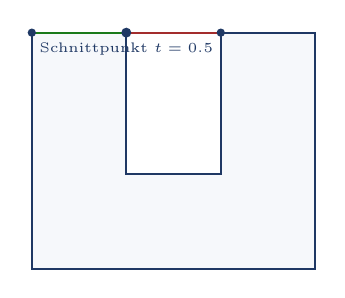
\begin{tikzpicture}[scale=0.6]
        % U-Polygon
        \fill[lightblue!40] (0,0)--(6,0)--(6,5)--(4,5)--(4,2)--(2,2)--(2,5)--(0,5)--cycle;
        \draw[darkblue,thick] (0,0)--(6,0)--(6,5)--(4,5)--(4,2)--(2,2)--(2,5)--(0,5)--cycle;
        % Teilsegment 1 (innen)
        \draw[mygreen, thick] (0,5)--(2,5);
        % Teilsegment 2 (außen)
        \draw[myred, thick] (2,5)--(4,5);
        % Schnittpunkt
        \fill[darkblue] (2,5) circle (3pt);
        \node[darkblue, font=\tiny, below] at (2,5) {Schnittpunkt $t=0.5$};
        % Endpunkte
        \fill[darkblue] (0,5) circle (2.5pt);
        \fill[darkblue] (4,5) circle (2.5pt);
      \end{tikzpicture}\\[0.2em]
      \small Mid2 bei $t=0.75$: $(3,5)$ liegt außen\\
      $\Rightarrow$ \textcolor{mygreen}{\textbf{nicht sichtbar}} — korrekt
    \end{column}
  \end{columns}
  \vspace{0.5em}
\end{frame}


% ============================================================
\section{SAT-Encoding}
% ============================================================

\begin{frame}{Guard-Variablen \& Coverage-Klauseln}
  \begin{block}{Guard-Variable}
    Für jeden Kandidaten $p_i \in P$:
    \[
      \guard{i} \in \{0,1\}, \quad
      \guard{i}=1 \iff p_i \text{ wird als Guard eingesetzt}
    \]
  \end{block}
  \vspace{0.3em}
  \begin{block}{Coverage-Klausel (pro Witness $p_j$)}
    \[
      \forall j:\quad \bigvee_{\substack{i \\ V[i][j]=1}} \guard{i}
    \]
    Mindestens ein Guard, der $p_j$ sieht, muss aktiv sein.
  \end{block}
  \vspace{0.3em}
  \begin{alertblock}{Coverage allein reicht nicht}
    Triviale Lösung: alle $\guard{i}=1$ erfüllt alle Klauseln.
    $\Rightarrow$ Kardinalitätsbeschränkung nötig.
  \end{alertblock}
\end{frame}

\begin{frame}{Kardinalitätsbeschränkung: $\sum \guard{i} \leq k$}
  \begin{itemize}
    \item SAT kennt keine Summation — nur boolesche Disjunktionen
    \item Die Schranke muss also über Klauseln simuliert werden
  \end{itemize}
  \vspace{0.6em}
  \begin{block}{Sequential Counter Encoding}
    Simuliert einen Zähler über Hilfsvariablen $\svar{i}{j}$.\\[0.3em]
    $\mathcal{O}(n \cdot k)$ zusätzliche Variablen und Klauseln —
    skaliert linear in $n$ und $k$, allgemein einsetzbar.
  \end{block}
  \vspace{0.8em}
  $\Rightarrow$ Diese Arbeit verwendet den \textbf{Sequential Counter}.
\end{frame}

\begin{frame}{Sequential Counter: Hilfsvariable \& Initialisierung}
  \begin{block}{Hilfsvariable}
    \[
      \svar{i}{j} = 1 \iff \text{unter den ersten } i \text{ Kandidaten sind mindestens } j \text{ Guards aktiv}
    \]
    \small Beispiel: $\svar{5}{2}=1$ bedeutet: unter $\guard{1},\ldots,\guard{5}$ sind mindestens 2 Guards aktiv.
  \end{block}
  \vspace{0.5em}
  \textbf{Initialisierung ($i=1$):} Äquivalenz $\svar{1}{1} \leftrightarrow \guard{1}$
  \vspace{0.3em}
  \begin{columns}[T]
    \begin{column}{0.48\textwidth}
      \small $\guard{1}=1 \Rightarrow \svar{1}{1}=1$\\
      Implikation: $\guard{1} \to \svar{1}{1}$
      \[
        \neg\guard{1} \vee \svar{1}{1}
      \]
    \end{column}
    \begin{column}{0.48\textwidth}
      \small $\svar{1}{1}=1 \Rightarrow \guard{1}=1$\\
      Implikation: $\svar{1}{1} \to \guard{1}$
      \[
        \neg\svar{1}{1} \vee \guard{1}
      \]
    \end{column}
  \end{columns}
  \vspace{0.3em}
  \small Beide Klauseln zusammen erzwingen die Äquivalenz —
  ohne Richtung 2 könnte der Solver $\svar{1}{1}$ frei setzen.
\end{frame}

\begin{frame}{Herleitung: Monotonie \& Inkrement}
  \begin{block}{Monotonie}
    \textbf{Regel:} Sind unter den ersten $i{-}1$ Kandidaten schon $\geq j$ Guards aktiv,
    gilt das auch für die ersten $i$.\\[0.2em]
    Implikation: $\svar{i-1}{j} \rightarrow \svar{i}{j}$
    \quad($a \to b \equiv \neg a \vee b$)
    \[
      \neg\svar{i-1}{j} \vee \svar{i}{j}
    \]
  \end{block}
  \begin{block}{Inkrement}
    \textbf{Regel:} Sind unter den ersten $i{-}1$ Kandidaten $\geq j{-}1$ Guards aktiv
    \emph{und} wird $\guard{i}$ zusätzlich gewählt, sind es $\geq j$.\\[0.2em]
    Implikation: $\svar{i-1}{j-1} \wedge \guard{i} \rightarrow \svar{i}{j}$
    \quad($(a{\wedge}b){\to}c \equiv \neg a \vee \neg b \vee c$)
    \[
      \neg\svar{i-1}{j-1} \vee \neg\guard{i} \vee \svar{i}{j}
    \]
  \end{block}
\end{frame}

\begin{frame}{Herleitung: Obergrenze}
  \begin{block}{Obergrenze}
    \textbf{Regel:} Mehr als $k$ Guards sind verboten. Sind unter den ersten
    $i{-}1$ Kandidaten schon $k$ Guards aktiv ($\svar{i-1}{k}=1$), darf $\guard{i}$
    nicht mehr aktiviert werden.\\[0.2em]
    Implikation: $\svar{i-1}{k} \rightarrow \neg\guard{i}$
    \quad$\equiv$\quad $\neg(\svar{i-1}{k} \wedge \guard{i})$
    \[
      \alert{\neg\svar{i-1}{k} \vee \neg\guard{i}}
    \]
    Das ist die eigentliche Schranke $\sum_i \guard{i} \leq k$.
  \end{block}
  \vspace{0.3em}
  \begin{center}
    \small
    \begin{tabular}{lll}
      \toprule
      \textbf{Idee} & \textbf{Implikation} & \textbf{CNF} \\
      \midrule
      Monotonie & $\svar{i-1}{j} \to \svar{i}{j}$ & $\neg\svar{i-1}{j} \vee \svar{i}{j}$ \\
      Inkrement & $\svar{i-1}{j-1}\wedge\guard{i} \to \svar{i}{j}$ & $\neg\svar{i-1}{j-1}\vee\neg\guard{i}\vee\svar{i}{j}$ \\
      Obergrenze & $\svar{i-1}{k} \to \neg\guard{i}$ & $\neg\svar{i-1}{k}\vee\neg\guard{i}$ \\
      \bottomrule
    \end{tabular}
  \end{center}
  \vspace{0.2em}
  \small Initialisierung wurde bereits gezeigt — Äquivalenz $\svar{1}{1} \leftrightarrow \guard{1}$ macht den Start des Zählers korrekt.
\end{frame}

% ============================================================
\section{Iteratives Lösen mit Kissat}
% ============================================================

\begin{frame}{Iteratives Lösen: Ablauf}
  \begin{enumerate}
    \item Starte mit $k=1$
    \item Erzeuge CNF: Coverage-Klauseln $\wedge$ Sequential Counter $(\leq k)$
    \item Kissat löst die Instanz
    \item Falls \textbf{UNSAT}: $k \leftarrow k+1$, zurück zu Schritt 2
    \item Erstes \textbf{SAT}-Ergebnis $\Rightarrow$ $k$ ist minimal
  \end{enumerate}
  \vspace{0.6em}

\end{frame}

 

% ============================================================
\section{MaxSAT-Encoding}
% ============================================================

\begin{frame}{Von SAT zu MaxSAT}
  \begin{alertblock}{Motivation}
    Iteratives SAT: im schlimmsten Fall $k_{\min}$ Solver-Aufrufe,
    jeder UNSAT-Nachweis teurer als der vorherige.
  \end{alertblock}
  \vspace{0.6em}
  \textbf{MaxSAT} formuliert Minimierung direkt:
  \begin{itemize}
    \item \textbf{Hard Clauses:} müssen erfüllt sein — Coverage-Klauseln
    \item \textbf{Soft Clauses:} sollen erfüllt sein, mit Gewicht — Verletzungen werden minimiert
  \end{itemize}
  \vspace{0.5em}
  \begin{block}{AGP als MaxSAT}
    \[
      \text{Hard:}\quad \bigvee_{i:\,V[i][j]=1} \guard{i} \quad \forall j
      \qquad\quad
      \text{Soft (Gewicht 1):}\quad \neg\guard{i} \quad \forall i
    \]
    Jede verletzte Soft Clause ($\guard{i}=1$) kostet 1.\\
    Solver minimiert Kosten $=$ Anzahl aktiver Guards.\\
    \alert{Keine Hilfsvariablen, kein iteratives $k$.}
  \end{block}
\end{frame}

\begin{frame}{WCNF-Format: konkretes Beispiel (L-Polygon, $|P|=8$)}
  \begin{columns}[T]
    \begin{column}{0.54\textwidth}
      \texttt{\small
        c AGP MaxSAT, L-Polygon \\[0.2em]
        \textcolor{mygreen}{h} 1 2 3 6 7 8 0\quad\textcolor{gray}{\% Cov.\ $p_2$}\\
        \textcolor{mygreen}{h} 3 4 5 6 7 8 0\quad\textcolor{gray}{\% Cov.\ $p_4$}\\
        \textcolor{mygreen}{h} 1 3 4 5 6 7 8 0\quad\textcolor{gray}{\% Cov.\ $p_5$}\\
        \quad\ldots\\[0.3em]
        \textcolor{amber}{1} {-1} 0\quad\textcolor{gray}{\% Soft: $\neg\guard{1}$}\\
        \textcolor{amber}{1} {-2} 0\quad\textcolor{gray}{\% Soft: $\neg\guard{2}$}\\
        \quad\ldots\\
        \textcolor{amber}{1} {-8} 0\quad\textcolor{gray}{\% Soft: $\neg\guard{8}$}\\
      }
    \end{column}
    \begin{column}{0.42\textwidth}
      \begin{block}{Legende}
        \textcolor{mygreen}{\texttt{h}} = Hard Clause (Coverage)\\
        \textcolor{amber}{\texttt{1}} = Soft Clause, Gewicht 1\\[0.5em]
        MaxHS minimiert:\\
        $\sum_i \mathbf{1}[\guard{i}=1]$\\
        $=$ Anzahl aktiver Guards
      \end{block}
      \vspace{0.4em}
      \small
      Lösung: MaxHS setzt $\guard{3}=1$,\\
      alle anderen $=0$\\
      $\Rightarrow$ Kosten $= 1 = k_{\min}$\\
      (auch $\guard{6},\guard{7},\guard{8}$ optimal)
    \end{column}
  \end{columns}
\end{frame}

\begin{frame}{Kissat (iterativ) vs.\ MaxHS (direkt)}
  \centering
  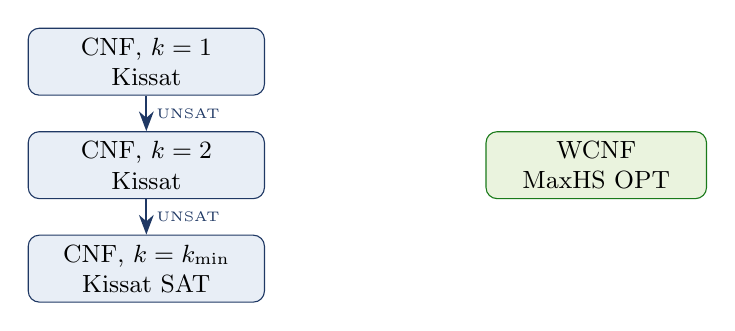
\begin{tikzpicture}[
      node distance=0.45cm and 1.5cm,
      box/.style={rectangle, rounded corners, draw=darkblue, fill=lightblue,
                   minimum width=3.0cm, minimum height=0.85cm, align=center, font=\small},
      arrow/.style={-{Stealth[length=2.5mm]}, thick, darkblue}
    ]
    \node[box] (k1) {CNF, $k=1$\\Kissat};
    \node[box, below=of k1] (k2) {CNF, $k=2$\\Kissat};
    \node[box, below=of k2] (k3) {CNF, $k=k_{\min}$\\Kissat \alert{SAT}};
    \node[box, right=2.8cm of k2, fill=lightgreen, draw=mygreen, minimum width=2.8cm] (max)
      {WCNF\\MaxHS \alert{OPT}};

    \draw[arrow] (k1) -- node[right, font=\tiny] {UNSAT} (k2);
    \draw[arrow] (k2) -- node[right, font=\tiny] {UNSAT} (k3);
  \end{tikzpicture}
  \vspace{0.8em}
  \begin{columns}[T]
    \begin{column}{0.48\textwidth}
      \textbf{Kissat:} mehrere kleine CNF-Instanzen\\
      Vorteil bei kleinem $k_{\min}$ (wenige UNSAT-Runden)
    \end{column}
    \begin{column}{0.48\textwidth}
      \textbf{MaxHS:} eine WCNF-Instanz\\
      Vorteil bei großem $k_{\min}$ (viele teure UNSAT-Nachweise entfallen)
    \end{column}
  \end{columns}
\end{frame}

% ============================================================
\section{Polygon-Klassen}
% ============================================================

\begin{frame}{Polygon-Klassen: Was macht sie für SAT schwer?}
  \begin{columns}[T]
    \begin{column}{0.48\textwidth}
      \textbf{\texttt{comb\_N}: Kammstruktur}\\[0.4em]
      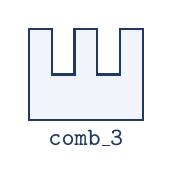
\begin{tikzpicture}[scale=0.58]
        \fill[lightblue!60]
          (0,0)--(0,2)--(0.5,2)--(0.5,1)--(1,1)--(1,2)--
          (1.5,2)--(1.5,1)--(2,1)--(2,2)--(2.5,2)--(2.5,0)--cycle;
        \draw[darkblue, thick]
          (0,0)--(0,2)--(0.5,2)--(0.5,1)--(1,1)--(1,2)--
          (1.5,2)--(1.5,1)--(2,1)--(2,2)--(2.5,2)--(2.5,0)--cycle;
        \node[font=\small, darkblue] at (1.25,-0.4) {\texttt{comb\_3}};
      \end{tikzpicture}
      \vspace{0.3em}
      \begin{itemize}
        \item Jede Zacke braucht eigenen Guard
        \item $k_{\min} = N$ — wächst linear
        \item Kissat: $N{-}1$ UNSAT-Nachweise, Kosten explodieren
        \item MaxHS löst direkt in konstanter Zeit
      \end{itemize}
    \end{column}
    \begin{column}{0.48\textwidth}
      \textbf{\texttt{random\_N\_seedM}: Zufallspolygon}\\[0.4em]
      
\begin{tikzpicture}[scale=0.58]
        \fill[lightblue!60]
          (0.3,1.8)--(1.0,2.2)--(1.9,1.7)--(2.3,0.9)--
          (1.8,0.1)--(0.9,0.0)--(0.1,0.6)--cycle;
        \draw[darkblue, thick]
          (0.3,1.8)--(1.0,2.2)--(1.9,1.7)--(2.3,0.9)--
          (1.8,0.1)--(0.9,0.0)--(0.1,0.6)--cycle;
        \node[font=\small, darkblue] at (1.2,-0.4) {\texttt{random\_10}};
      \end{tikzpicture}
      \vspace{0.3em}
      \begin{itemize}
        \item Optimum oft klein ($k=1$ oder $k=2$)
        \item Kissat: wenige UNSAT-Runden nötig
        \item MaxHS trägt Overhead der Soft-Clause-Optimierung
        \item Kandidatenanzahl wächst stark mit $N$
      \end{itemize}
    \end{column}
  \end{columns}
\end{frame}

\begin{frame}{Benchmark-Setup}
  \begin{itemize}
    \item \textbf{Instanzen:} \texttt{comb\_3} bis \texttt{comb\_6};
          \texttt{random\_10-30\_seed1--5}
    \item \textbf{Zweistufiges Benchmarking:}
      \begin{enumerate}
        \item Preprocessing-Phase: Kandidaten + Sichtbarkeit berechnen,
              CNF/WCNF erzeugen und cachen
        \item Solve-Phase: reine Solver-Zeit auf gecachten Dateien messen
      \end{enumerate}
    \item \textbf{Kandidatengenerierung:} 0, 1, 2 Runden
    %\item \textbf{Zeitlimit:} 120\,s pro Solver-Aufruf
  \end{itemize}
  \vspace{0.3em}
\end{frame}


% ============================================================
\section{Ergebnisse}
% ============================================================
 
\begin{frame}{Beispiellösungen: Sichtbarkeitsgraph \& Guards}
  \centering
  \begin{columns}[T]
    \begin{column}{0.48\textwidth}
      \centering
      \includegraphics[width=0.92\textwidth]{../plots/comb_3.pdf}\\[0.3em]
      {\footnotesize \texttt{comb\_3}: optimale Lösung, $k_{\min}=3$ Guards}
    \end{column}
    \begin{column}{0.48\textwidth}
      \centering
      \includegraphics[width=0.92\textwidth]{../plots/random_20_seed1.pdf}\\[0.3em]
      {\footnotesize \texttt{random\_20\_seed1}: optimale Lösung, $k_{\min}=2$ Guards}
    \end{column}
  \end{columns}
  \vspace{0.4em}
  \small Sichtbarkeitsgraph aller Kandidaten mit gewählten Guards (rot)
  und ihrer Abdeckung.
\end{frame}
 
\begin{frame}{Einfluss der Rundenzahl: \texttt{comb}}
  \begin{center}
    \includegraphics[width=0.92\textwidth]{../plots/comb_vs_rounds.pdf}\\[0.2em]
  \end{center}
\end{frame}
 
\begin{frame}{Einfluss der Rundenzahl: \texttt{random}}
  \begin{center}
    \includegraphics[width=0.92\textwidth]{../plots/random_vs_rounds.pdf}\\[0.2em]

  \end{center}
\end{frame}
 
\begin{frame}{Ergebnisse: UNSAT-Explosion bei \texttt{comb}}
  \begin{center}
    \includegraphics[width=0.78\textwidth]{../plots/comb_per_k_r2.pdf}\\[0.3em]
    {\footnotesize Kissat-Zeit pro $k$-Aufruf (log-Skala, \texttt{rounds=2}).
    Bei \texttt{comb\_6} erreicht der UNSAT-Nachweis für $k{=}4$
    bereits das Zeitlimit --- Optimum $k{=}6$ wird nie erreicht.}
  \end{center}
\end{frame}
 
\iffalse
\begin{frame}{Ergebnisse: Tabelle}
  \centering\small
  \begin{tabular}{lcccc}
    \toprule
    \textbf{Instanz} & \textbf{$k_{\min}$} & \textbf{MaxHS (s)}
                     & \textbf{Kissat (s)} & \textbf{Kissat-Calls} \\
    \midrule
    \texttt{comb\_3} & 3 & 0.18 & 0.04 & 3 \\
    \texttt{comb\_4} & 4 & 0.10 & 0.22 & 4 \\
    \texttt{comb\_5} & 5 & 0.07 & 51.05 & 5 \\
    \texttt{comb\_6} & 6 & 0.34 & \textcolor{myred}{129.54 (Timeout)} & 4 \\
    \midrule
    \texttt{random\_10\_seed1} & 1 & 0.09 & 0.01 & 1 \\
    \texttt{random\_20\_seed1} & 2 & 1.85 & 0.46 & 2 \\
    \texttt{random\_20\_seed2} & 2 & 4.91 & 0.56 & 2 \\
    \midrule
    \texttt{random\_30\_seed3} & 2 & \textcolor{amber}{72.59} & 9.16 & 2 \\
    \bottomrule
  \end{tabular}\\[0.8em]
  {\footnotesize Vollständige Tabelle (15 Instanzen) im Code-Repository.
  \texttt{random\_30}: MaxHS deutlich langsamer als bei kleineren Instanzen ---
  Kandidatenanzahl treibt auch die WCNF-Größe.}
\end{frame}

\fi
 
% ============================================================
\section{Diskussion}
% ============================================================



% ============================================================
\section{Fazit \& Ausblick}
% ============================================================

\begin{frame}{Fazit \& Ausblick}
  \begin{block}{Zusammenfassung}
    \begin{itemize}
      \item AGP erfolgreich als SAT (Sequential Counter) und MaxSAT (WCNF) enkodiert

    \end{itemize}
  \end{block}
  \begin{block}{Ausblick}
    \begin{itemize}
      \item \textbf{Kandidatengenerierung} ist Flaschenhals bei großen Instanzen
            (\texttt{random\_30}: Vorverarbeitung sprengt Zeitlimit)
            $\Rightarrow$ Optimierungspotenzial als nächster Schritt
      \item \textbf{Rundenvergleich}: 1 vs.\ 2 vs.\ mehr Runden — bessere Optima?
    \end{itemize}
  \end{block}
\end{frame}

\begin{frame}{}
  \centering
  \Large Vielen Dank!\\[1em]
  \normalsize Fragen?
\end{frame}

\end{document}